\documentclass[12pt]{article}
\usepackage[normalem]{ulem}
\usepackage{graphicx, multirow}
\usepackage{amsmath, array}
\usepackage{fancyheadings, lastpage}
\usepackage{pdflscape ,anyfontsize}
\usepackage{longtable}
\usepackage{titlesec}
\usepackage{filecontents}
\usepackage{listings}
\usepackage{algpseudocode}
\usepackage{pdfpages}
\usepackage[a4paper]{geometry}
% REFERENCE http://tex.stackexchange.com/questions/4891/how-do-i-control-the-spacing-above-a-new-paragraph %
\makeatletter
\renewcommand{\paragraph}{
  \@startsection{paragraph}{4}
  {\z@}{3.25ex \@plus -10em \@minus 1em}{0.1em}
  {\normalfont\normalsize\bfseries}
}
\lstset{
    breaklines=true,
  }
\makeatother
\setcounter{secnumdepth}{5}
\setcounter{tocdepth}{6}
\renewcommand{\refname}{}
\renewcommand{\headrulewidth}{0pt}
\lhead{Group Project 07 - Final Report}
\rhead{(Draft) -Version 2.2}
\lfoot{Aberystwyth University / Computer Science}
\cfoot{}
\rfoot{\thepage{}  of  \pageref{LastPage}}
\usepackage{graphicx}
\begin{document}
\pagestyle{fancy}
\begin{flushleft}
\rule[0.2cm]{13.8cm}{0.02cm}
\end{flushleft}
{\fontsize{20}{20}\selectfont \textbf {\centerline{Group Project 07 Final Report}}}
\begin{flushleft}
\rule[0.2cm]{13.8cm}{0.02cm}
\end{flushleft}

\begin{tabular}{ l l }

\\ \multirow{1}{*}{\textit{Authors: }} & Mosopefoluwa David Adejumo \\  & Ryan Gouldsmith \\
& Harry Flynn Buckley \\ & Zack Lott \\ & Mark Radcliffe Pitman \\ & Jack Alexander Reeve \\ & Mark Alexander Smith \\ &Martin Vasilev Zokov \\ & Maciej Wojciech Dobrzanski \\
\\ \multirow{1}{*}{\textit{Config ref: }} & SE\_07\_FR\_01 \\
\\ \multirow{1}{*}{\textit{Date} } & \today \\
\\ \multirow{1}{*}{\textit{Version}} & 2.2 \\ 
\\ \multirow{1}{*}{\textit{Status}} & Draft \\

\end{tabular}


\vspace{3.2cm}
\hfill\begin{minipage}{\dimexpr\textwidth-0.3cm}
Department of Computer Science \\
Aberystwyth University \\
Aberystwyth \\
Ceredigion\\
SY23 3DB \\
Copyright \small{\copyright}\\ Aberystwyth University 2013
\end{minipage}

\newpage
\tableofcontents{}

\newpage
\section{INTRODUCTION}
\subsection{Purpose}
This document contains a report of all the events and status of the project and is a compilation of all the documents used.
\subsection{Scope}
This document should be read by all members of the group for approval. It contains an overall evaluation of every group member and the details of the project, its final state with details of all the events of the project. There is also maintenance manuals for each of the different applications. Therefore, enclosed is a manual for the Android application, Web Application and Database implementation - each give key points on how to maintain each piece of software. Finally, there are the test log, design specification and Project Plan included in this document as appendices. 
\subsection{Objective}
\begin{itemize}
\item Provide a historical account of events during the project
\item Provide a report on how all the members performed and the team
\item Provide a report from every member about how they feel they performed
\item Provide a compilation of all documents used for development and planning
\item Provide details on how to maintain the project for future use
\end{itemize}
\newpage
\section{THE END-OF-PROJECT REPORT}
\subsection{Management}
The program satisfied most of the basic requirements. On the website, all the requirements were met and the user is able to view walks and their associated information including images, points of interest and the path of a walk. However on the Android, while the user is able to upload and record walks as well as edit the name of the walk and its descriptions, the Android application had a bug where it would crash after uploading a walk instead of returning to the home screen. This bug was identified before submission, however, a fix was found after the submission deadline, and thus not implemented in the final product. Users were also unable to edit or remove individual points of interest once created and thus to remove a point of interest, the walk had to be restarted. 
\\\\
There was also heavy feature creep much of which was removed from the final product. The feature creep resulted in time being wasted on features that were cut. One main issue was displaying a map on the Android this was going to be used to display points of interest and allow editing of points of interest, but was cut due to difficulties in implementation. There was also an issue where the development on the website stagnated. This lack of progress led to the website being off schedule. Extra work was performed by the QA Manager to bring us back on schedule. A third issue was issues with decoding the JSON data on the server. To allow us to see what data was being sent, we created a log file and used it to assist in the coding of the decoder. Images were also converted to a string and decoded using base64.
\\\\
Overall, the team performed well, however the lack of progress on the web team caused issues late in development and the tasks had to be reorganized. The Android programmers performed exceptionally well, remaining on schedule. However, the manager spent times focusing on several areas particularly during coding week and so several members would occasionally cease to do work, having not been assigned a task. There were issues with Github not tracking the number of commits made by members, despite showing these commits in the log.
\\\\
Below is an example of a weekly report. This report is a summary of work done as the actual reports provided by the members were more detailed
\begin{figure}
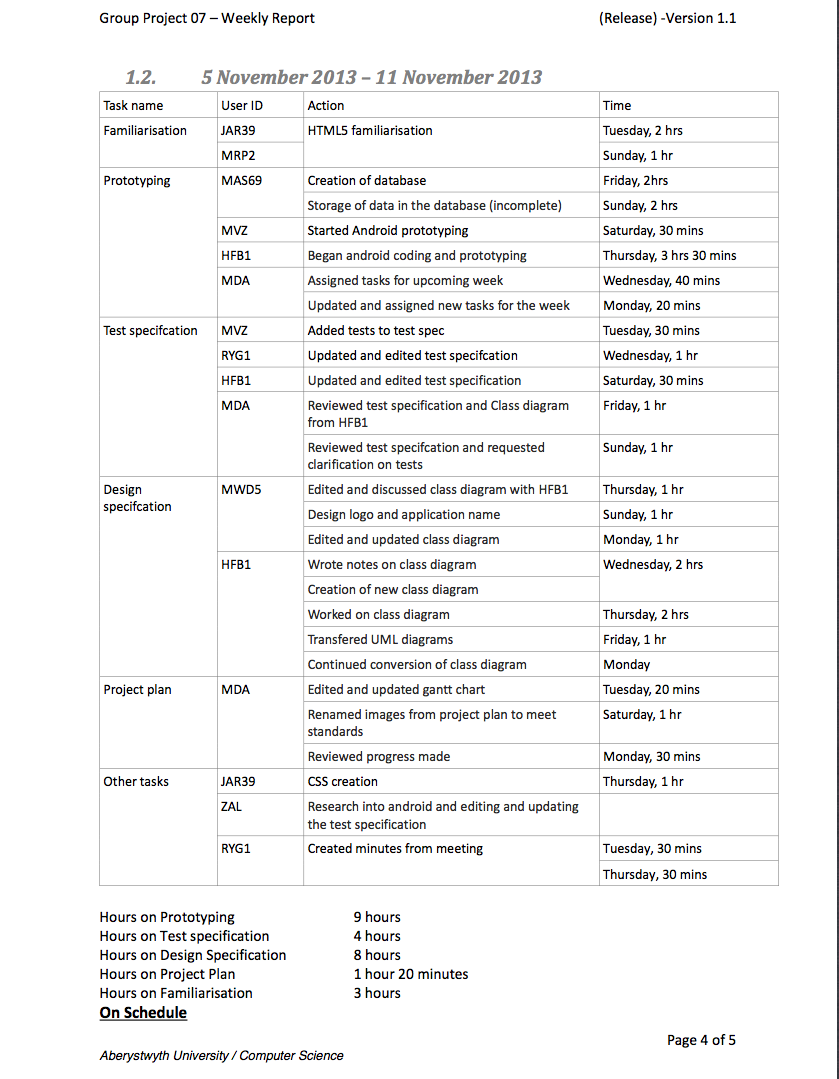
\includegraphics[scale=0.60]{Final_report/weekly_report.png}
\caption{Example of a weekly report.}
\end{figure}
\newpage
\subsection{History}
At the start of the project, the group were all required to produce reports of all work performed during the week which was usually a summary of the blog. These reports were submitted to the project manager to ensure the project remained on schedule. Planning began immediately and the project manager made several revisions to the Gantt chart and one of the members requested a change of roles which was included in the Gantt chart. During the design phase we wanted the walks to record actual user movement and not a direct point to point depiction of the walk. This meant storing more cooridnate information in the database. We used the term Point of Interest (POI) to refer to locations where the user added a description or images. These points of interest would be where markers are displayed on the website, with locations simply being coordinates. I.e. A Location is a set of coordinates while a point of interest is a location with more info such as a description and images.
\\\\
The project plan was produced during a meeting in which all members suggested the initial design of the system and their understanding of the requirements. MDA typed the document and used images created by MWD5 and JAR39. Subsequent documents were produced as a contributed effort where different members worked on their specialized areas. I.e the web programmers worked on the website aspect of the design specification, while the android programmers worked on the Android aspect. The class diagram was produced by HFB1 and approved by MDA. There was also a lack of Android devices in the group particularly among the Android programmers, so several members decided to purchase their own devices. Android emulators were avoided as their relatively poor performance meant that they impractical.
\\\\
During the process of the project, meetings were held twice weekly, one on Tuesday's with the Project Supervisor and a second on Fridays to discuss work during the week and goals for the next Tuesday meeting. These meetings helped identify and eliminate feature creep in some areas, but also resulted in the addition of feature creep in other areas. These meetings also were used to discuss changes in design before coding. One such instance was the use of the OpenSpace API. It was during a meeting that one of the Android programmers MVZ notified the project manager of the inefficiencies of the API and this resulted in the switch from OpenSpace to Google Maps API.
\\\\
During prototyping, several issues were encountered but allowed certain design decisions to be made early. Production of the website prototype had several issues. These included the lack of any dynamic code (PHP). However there was a map present in the website, and an idea of the behaviour of the website was given through the prototype. The Android progressed further during prototyping in which core features including basic navigation through screens and uploading text data were operational. However, the prototype did contain features which were removed later during development. The web based prototype was hosted on MVZ's public html. It was not hosted on the web programmers filestore because of an assignment for a web module as we wanted to avoid the possibility of modifying the permissions of the web assignment files thereby causing a late submission.
\\\\
Creation of the database also proved difficult, due to the decision to host it on the universities network. There were issues with creating the database but after enquiries by MAS69, the database was created but didn't have any data. Due to an ongoing assignment, several group members were unable to focus on the group project. The project manager, who didn't have any required assignments at the time, created a web based interface which was used to create and delete tables with ease. Over the Christmas holiday, RYG1 created a simple interface for manually adding information in the database as well as modifying a file which displayed all the information in the database. These scripts were later used extensively for testing. However by the start of the second semester, the database tables were not being joined correctly.
\\\\
During the Christmas holiday, RYG1 worked extensively on the website producing the basic files for the website, however the server still had no means of putting data in the database tables. The Android development also proceeded at a fair pace during this time, with the walk recorder being implemented. However, image uploading was not functional at the time. 
\\\\
After completion of the exams, a meeting was held to discuss plans for Integration and Coding Week and all progress made over the Christmas holiday. Integration and coding week saw all group members working from 9am to about 5pm or 6pm. The first day of the week saw the implementation of uploading basic walk information and elimination of all feature creep that had arisen during the planning stage. There were difficulties in reading the JSON data on the server and this led to the creation of a log file which proved useful for further development. By Tuesday, the website still was not functional to an acceptable state however the web programmers had developed code which turned out to only be functional for hard coded data. In order to increase the website development, the project manager began working on the file\_saver.php file which handled the data being received from the Android device. MAS69 assisted MDA in finding a tutorial on how to extract variables from the JSON data. 
\\\\
RYG1 was put on full website development and the website was moved to MDA's public html as project leader, while MWD5 began producing JUnit tests while ZAL also produced PHPUnit tests. Initially these were to be used for the file\_saver.php file, but lack of knowledge led to the removal of several tests. The project manager worked extensively on the file\_saver.php file on Tuesday and Wednesday and was able to add information to the database, however joining the tables was solved by RYG1. On the Android a conflict arose where the Android programmers had mapped the same button to different functions. While this initially was not seen as a major issue, MVZ was instructed to create a screen to override the button conflict. This presented an issue where the buttons on the screen were not functioning. This was solved by the project manager who passed the variables as required and this fix in turn solved another similar bug that had appeared elsewhere. By Wednesday, RYG1 had to refactor all the website code to bring in correct functionality and thus the remaining members of the web team were moved into production of CSS files and testing the walks. \\\\
By Thursday, at the suggestion of the QA manager, the map being displayed on the Android was removed, due to group vote, although the project manager did not agree with such a move, it did help the project remain on schedule. By early morning, the website became fully operational, with the project manager displaying multiple images on the website when a point of interest is located. By this time, the Android satisfied most of the requirements, however during late testing a bug was discovered which caused the application to crash on upload. Friday morning was spent doing extensive bug fixing, testing and commenting code with Javadoc and PHP doc. The upload crash bug was partially solved, but the application began crashing after uploading. The project manager put a work deadline 15 minutes to the final deadline by which all work would stop. On submission, the group produced very little work during the next week, but the final documentation was completed shortly after a meeting on the week prior to the submission deadline.
\\\\
A major issue was misunderstanding the definition of MIME type and all images were converted to a string to decode. The image decoding had problems as decoders were unable to decode the text data. HFB1 used a text editor to remove backslashes which solved the problem so code was added to file\_saver.php to remove the escape slashes added by JSON.
\\\\
By the final week of documentation, development stagnated. MDA and RYG1 had to put in extra effort to see to the completion of the final document. However other members did contribute though not to the level of MDA and RYG1.
\newpage 
\subsection{Final State}
On the website, the project has been completed and the only known flaw was the map not displaying correctly on certain browsers. The website was tested on the following: Safari, Opera, Firefox, Internet Explorer, Google Chrome, Mobile Opera (Android), Android default browser and Mobile Safari (iPad). The following browsers had issues:\- Firefox: the map was displayed out of place on older versions, Android default browser: Did not display the map. All other features worked correctly, Internet Explorer: Some versions did not display the map, other versions displayed it out of place.
\\\\
The final website can be found here http://users.aber.ac.uk/mda/csgp07/wtc 
\newline
all other server based files including database testing files can be found here
\newline
http://users.aber.ac.uk/mda/csgp07 
\newline
(Login for database testing- Username: grp7admin Password: Wc7gp)
\\\\
The database had constraints applied to its data as required and walks were stored correctly on the website. The Android device crashed when uploading a large number of images or after a completed upload. The crash was possibly caused by the recorder only stopping the recording on completion of the upload. However the device iterates through the array of locations during upload. If there is a GPS signal during upload, the crash occurs due to data being added to the array during iteration through said array. The application also crashed when attempting to upload without a connection to the internet, however the crash may have been caused be the aforementioned bug and we were unable to isolate the cause.
\\\\
The user is also only able to edit the overall walk details: name, long and short descriptions. Individual points of interest cannot be edited once created. There is no indication of edit completion, however there is feedback when recording starts. The recording may also stop after 15 minutes of inactivity due to the Android device terminating the service. This is probably caused by the method used to implement the service. On successful uploads, the user is returned to the start screen however, due to the bug discovered late, the application may crash instead of returning the user to the start screen. 
\\\\
There may be several grammatical issues as of yet unidentified in the program. The GPS may also cut out leading to erratic lines when viewing a walk. This is a device and GPS issue and cannot be resolved by the application. Places, Locations and photo ID's are acquired by getting the ID of the last entry into the database, as a result, it may be possible to have details of a walk linked incorrectly if two or more walks are uploaded and processed within fractions of seconds from one another. However, we could not test this out and cannot verify as to whether or not it can occur. Any other errors have not been identified by the project members.
\\\\
There were several website files submitted which were not our own work. These files were used solely for early designing and prototyping.
The files that were not created by us are:
\begin{itemize}
\item all font files
\item all external javascript files
\item all files in the shadowbox-3.0.3 folder
\item all images in the Website/images folder
\item lightbox.css
\end{itemize}
\newpage
\subsection{Member Evaluation}
\subsubsection{Mosopefoluwa David Adejumo}
\centerline{\emph{Mosopefoluwa David Adejumo - MDA:} \textbf{Project Leader}}
~\\
MDA requested the creation of weekly reports to monitor group data and handed out tasks as well as oversaw the development of the project. Several aspects of feature creep were not identified or accounted for early on in planning which affected late development. Also occasionally put a lot of focus into single parts of the project resulting in slowed development in others. Development was brought back on schedule via task reorganisation. Also worked on the file\_saver.php file as well as displaying multiple images on the browser and minor bug fixing on the Android. Would send out emails regularly to group members requesting tasks be done. 
\subsubsection{Ryan Gouldsmith}
\centerline{\emph{Ryan Gouldsmith - RYG1:}\textbf{ Quality Assurance Manager}}
~\\
Oversaw the maintenance of standards in quality assurance. Assisted the project manager in overseeing the web programmers in development as well as performing extensive work on the website. Also worked on the Test Specification producing a large number of tests to be done. The QA performed well doing web development to keep the project on schedule and was easy to make contact with for the duration of the project. Also produced minutes for all the meetings when required. Reviewed the documents as required. Excellent performance throughout development.

\subsubsection{Harry Flynn Buckley}
\centerline{\emph{Harry Flynn Buckley - HFB1:}\textbf{ Android Programmer}}
~\\
Worked on Android coding. Developed the first prototype and worked on image integration of the Android application with both the camera and the library. Also integrated the uploading of the device and storing walks. Towards the end of coding week, he put a lot of effort into development and bug fixing in order to get the program to an acceptable state despite setbacks. Performed excellently throughout the project, and remained very active in keeping the project manager up to date with progress.

\subsubsection{Martin Vasilev Zokov }
\centerline{\emph{Martin Vasilev Zokov - MVZ:}\textbf{ Android Programmer}}
~\\
Worked on Android coding. Implemented the recording of walks as well as some GUI screens. Coded the algorithms for adding points of interest and recording the walk as well as GPS integration and recording checking. After completion of tasks, worked on bug fixing and Javadocs. Excellent performance throughout the project. Although there was an occasional loss of communication, work continued as expected keeping the project on schedule.

\subsubsection{Mark Alexander Smith}
\centerline{\emph{Mark Alexander Smith - MAS69:}\textbf{ Web Programmer}}
~\\
Saw the creation of the database and provided assistance in decoding the JSON data. Also worked on the base template of CSS in the final product and performed extensive testing. One particular field test proved extremely useful in development. Occassinally slowed down development wise, but would quickly pick up, keeping the project on schedule. Great performance throughout the project and would perform tasks in a timely manner.
\subsubsection{Jack Alexander Reeve}
\centerline{\emph{Jack Alexander Reeve
 - JAR39:}\textbf{ Web Programmer}}
~\\
Produced early prototypes of the website. Also produced the initial drawing of walks on maps between points of interest. Worked on CSS as well as website fixing and testing on different browsers. Also worked on the list walks.php file. Did lots of tidying up of the website, particularly towards the deadline. Excellent performance and produced most items on time. Difficult to reach between the start of the Christmas holidays and the semester starting week, but quickly made up for lost work.
\subsubsection{Mark Radcliffe Pitman}
\centerline{\emph{Mark Radcliffe Pitman - MRP2:}\textbf{ Web Programmer}}
~\\
Initially slow performance, and occasionally difficult to contact, worked on CSS of the final site as well as creation of the terms of service page. Picked up performance after the first day of coding week. Would perform tasks as soon as requested. Worked with other web programmers to produce CSS for the list walks page and also produced an early prototype for login page and worked on the website maps API. However this was not used as accounts were removed from the final project. Great performance during coding week. Also produced some PHP Unit tests when requested. Also worked on testing the website.
\subsubsection{Zack Lott}
\centerline{\emph{Zack Lott - ZAL:}\textbf{ Web Tester}}
~\\
Worked on the test specification and also produced a test report and worked on testing the website to ensure it met all the requirements. Also produced some PHP Unit tests which. Occasionally slowed down development during coding week. However this was due to lack of technical knowledge of PHP Unit testing. Picked up performance, once PHP Unit was learnt. Also did extensive field testing of the Android and testing of the website. Great performance particularly during coding week.
\subsubsection{Maciej Wojciech Dobrzanski}
\centerline{\emph{Maciej Wojciech Dobrzanski - MWD5:}\textbf{ Android Tester}}
~\\
Worked on the test specification. Was initially working solely on documents but requested to be moved to testing, to increase involvement in the group project. Was particularly eager to contribute and offered assistance where necessary or requested tasks to perform. Produced extensive JUnit tests and extensive Android testing and identification of bugs. Performed well and completed tasks in a timely manner throughout the project. Also produced several UML diagrams for the project. 
\newpage
\subsection{Team Evaluation}
As a team there were occasional issues mainly due to miscommunication or lack of communication. However, when all members were present and actively working together, development would progress rapidly as conflicts both program wise and personality wise were easily resolved. Consistent reports helped keep the project on schedule. However, communication could have been improved as there were issues that members had that the project leader would be unaware of, but would be notified eventually, usually during a meeting where the project supervisor was present. 
~\\\\
The team members collaborated with each other well, preventing an overlap of tasks and allowing development to proceed smoothly as well as helping keep feature creep out of the final product. If things were to improve, it would be to improve communication as that was the main issue with the group. Contacting each other was rarely the issue, it was mainly due to misinterpreting statements and sentences, possibly due to cultural differences of the members.
~\\\\
Tasks could also be monitored and better allocated to a more precise level and to take advantage of the strengths and weaknesses of each of the group members, with members sorting out issues with the affected members as needed.
~\\\\
The project also had issues with understanding the requirements and identifying feature creep. There was a large amount of feature creep initially and if these had been identified and removed earlier on, there may have been more time for bug fixing, and the Android may have been able to fully implement the requirements. Another issue was understanding and interpreting the requirements. Better contact or communication with the client should have been taken. This would have helped keep things to the point as the final product would better match what the client wanted as the specification given was vague in certain areas. This led to development of features or planning of features which were not required and thus time and spent or wasted performing those tasks.
~\\\\
It is important for members to work closely together and maintain communication and collaboration with each other. A project must be managed to a precise level and all problems should be taken up and sorted out with the appropriate person, be they the client or another member of the team. Also, in order to ensure a project is completed on time, the manager should assign tasks based on the feedback of the team members and the technical knowledge of such tasks. With a team it is fairly easy to run into conflicts in development due to poor communication and these can in turn have a greatly negative impact on the final product.
\newpage
\section{APPENDICES}
\subsection{The Project Test Report}
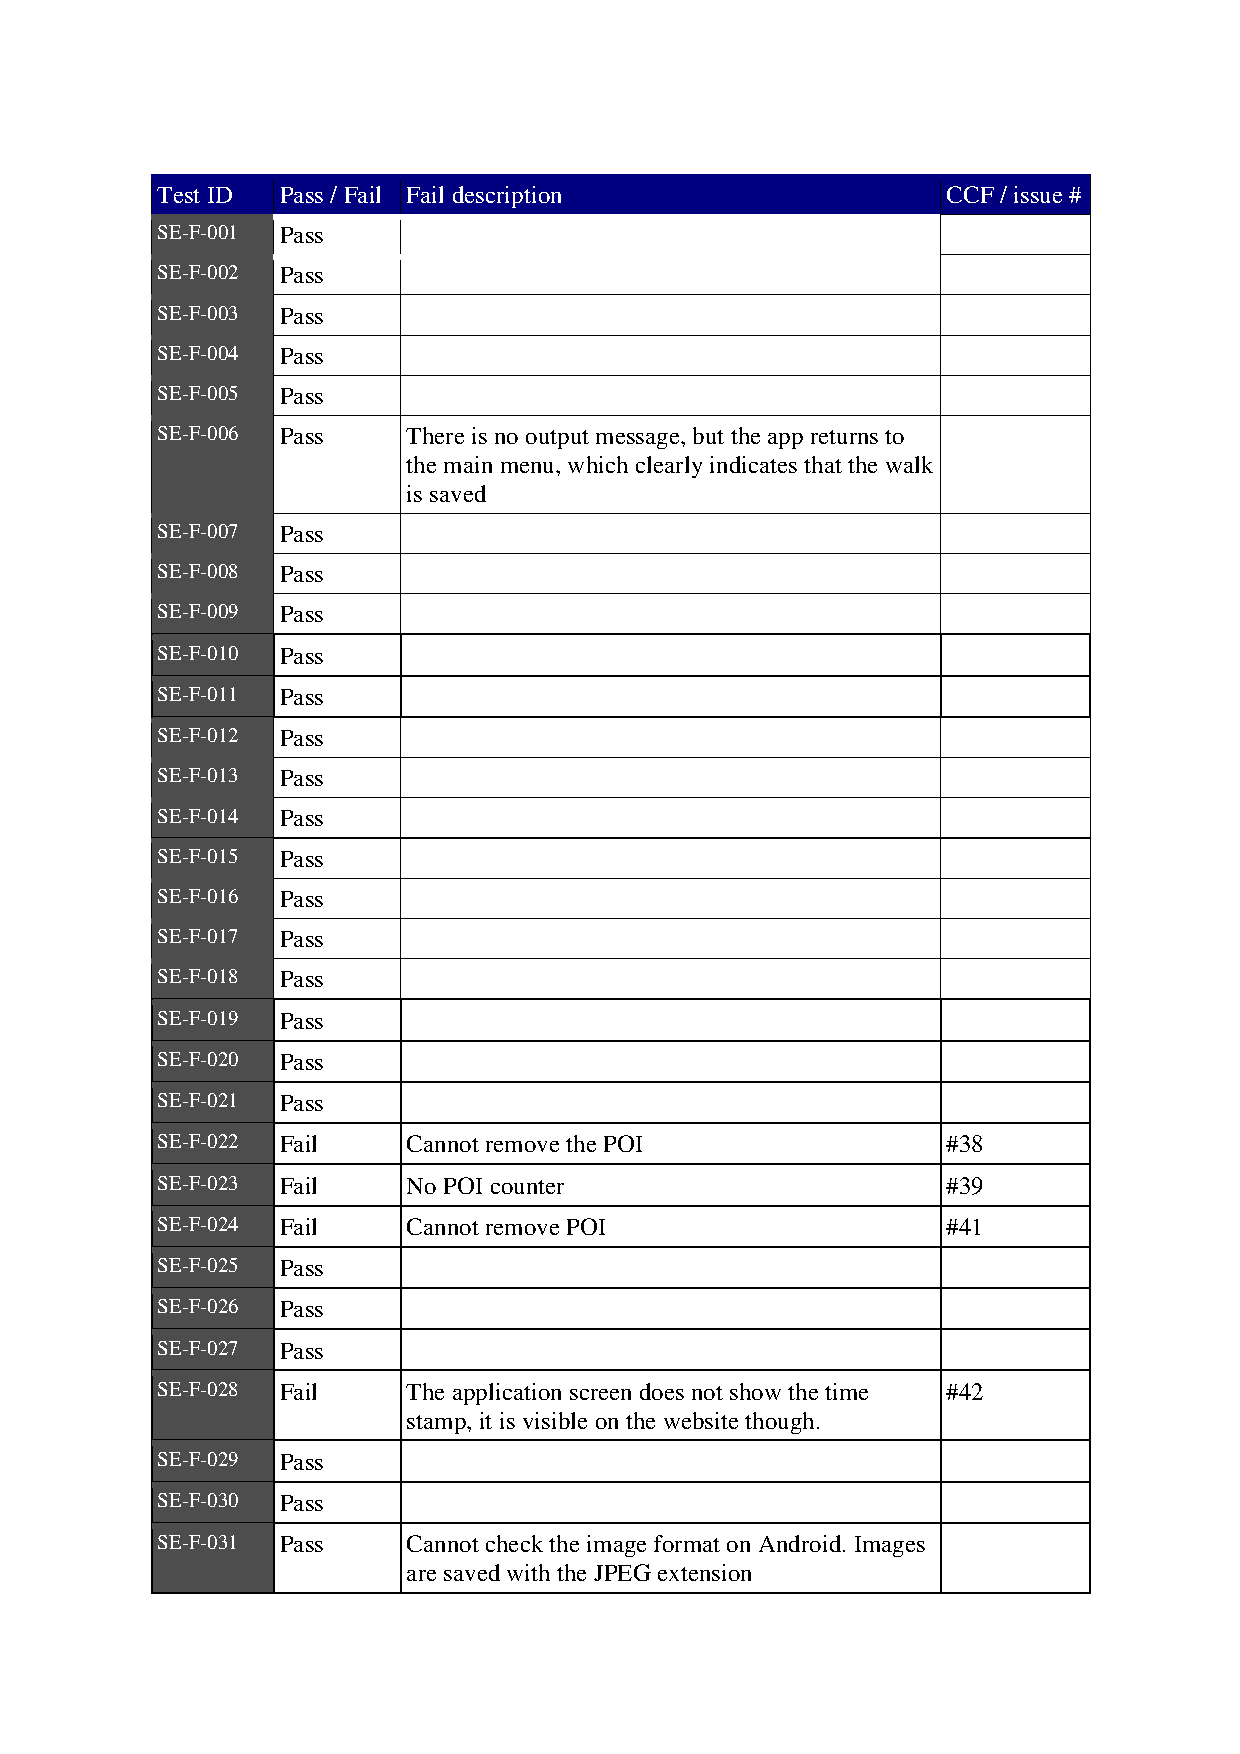
\includegraphics[scale=0.7]{testlog.pdf}
\includepdf[scale=0.7, pagecommand={}, pages=2-]{testlog.pdf}

\subsection{The Project Maintenance Manual}
\subsubsection{Android Maintenance}
\paragraph{Program Description}
The function of this program is to allow the user to document walks. The path of the walk is tracked by the GPS of the device and by tracking the GPS of the device and providing the user with the means add places of interest.
\paragraph{Program Structure}
The program is organised in to Android Activities classes that control the application until a new Activity is started.
\\\\
The initial activity that the used sees is the StartScreen, that presents the user with a button prompting the start of a new walk, this button will start a new activity that creates the walk.
\\\\
WalkSetupScreen allows the user to enter basic walk data such as title and description. This input is used to create a new walk.
The majority of  functionality is dealt with by the WalkScreen, it is responsible for the providing the user with options about the walk. From here places of interest can be created and added to the current walk.
\\\\
\textbf{Walk module}- This module handles all data about a walk - the route that was taken during the walk, the points of interest that were added and the information for the walk itself.
~\\
\textbf{Classes:} WalkModel, LocationPoint, PointOfInterest~\\\\
WalkModel stores the details of a walk. it uses three string variables for the title, short description and long description. It also keeps all the route data into a Vector of LocationPoint objects. The WalkModel object also calculates the distance traveled and the time spent on a walk.
~\\\\
LocationPoint objects are created when GPS data is received and the longitude and latitude are stored as well as a time stamp for the location.
~\\\\
PointOfInterest objects are inherited from the LocationPoint class and whenever a new POI is added. These objects have a Vector of ImageInformation objects that were added from either the camera or the gallery. PointOfInterest objects also have a title and a description. This information is added in the pop up dialog which is shown when the user adds a new PointOfInterest. The exact coordinates for the object are taken from the last known position, which is recorded in the RouteRecorder class.
~\\\\
\textbf{Recorder module}~\\
This module handles the recording and storing of route data.~\\
\textbf{Classes}: RouteRecorder, PositionListener~\\\\
RouteRecorder creates the LocationManager (Android API) and gives it a PositionListener object to respond to received GPS data. The listener then calls the newLocation method from the RouteRecorder to add it to the Vector of LocationPoints.~\\\\
The RouteRecorder keeps track of the last known position which is used when adding new points of interest. 
~\\\\
\textbf{Image module}~\\
This module is responsible for adding images to a walk. It is used to either get an image from the camera or select an image from the gallery on the device. ~\\
\textbf{Classes:} ImageHandler, ImageInformation
~\\\\ImageHandler uses two result codes to choose whether to start an activity to pick an image from the gallery or take a new picture.~\\\\
ImageInformation is used to store information for a single image. It is mainly used to encode the image information as a string in Base64 encoding and is then sent to the server.~\\\\
\textbf{File Transfer module}~\\
This module is responsible for sending~\\
\textbf{Classes:} FileTransferManager ~\\\\
FileTransferManager is responsible for packaging all the data for the current walk into a single JSON object that is then sent as an HTTP POST to a web server. It also has an inner class which is responsible for the upload. It starts in a new Thread in which the upload is handled.~\\\\
\textbf{Popup dialogues module}~\\
This module is used to display popup dialogues for various.~\\ 
\textbf{Classes:}DialogView, CancelWalkView, EditWalkView, GpsCheckDialog, PoiDialogView, WalkFinishedView~\\
All of these classes are essentially the same. They use the abstract class DialogView to create a default pop up window and show different layouts depending on the situation. Each of the popup classes uses a different layout that is defined in an XML file and displayed in the pop up. There is a listener which has a different implementation in each of the classes to respond to the button clicks in different ways.
~\\\\
CancelWalkView brings up a warning message that this action will delete all information about the walk.
~\\\\
EditWalkView gives options to set a different title, short and long descriptions for the current walk. A future improvement could be displaying the current title and descriptions for the walk.
~\\\\
GpsCheckDialog is displayed if the GPS on the device is not turned on and gives the user an option to go to the GPS settings and turn it on.
~\\\\
WalkFinishedView gives the option to stop the current walk, upload it and go back to the main screen of the application.
\paragraph{Significant Algorithms}
The methods below open up new screens
\\\\
public void finishWalk(View v)\{\}
\\\\
public void editWalkDialog(View v)\{\}
\\\\
public void cancelWalk(View v)\{\}
~\\\\
The below methods are related to the \textbf{Walk Model:}

public WalkModel() \{\}~\\
This is the default constructor for the WalkModel that creates the Vector for the route. ~\\\\
public String getTitle()\{\} ~\\
This gets the title of the walk ~\\\\
public void setTitle(String newTitle)\{\}~\\
This sets the title of the walk ~\\\\
public String getShortDescription()\{\}~\\
This gets the short description of the walk ~\\\\
public void setShortDescription(String newShortDesc)\{\}~\\
This sets the short description of the walk ~\\\\
public String getLongDescription()\{\}~\\
This gets the long description of the walk~\\\\
public void setLongDescription(String newLongDesc)~\{\}~\\
This sets the long description of the walk~\\\\
public Vector \textless LocationPoint \textgreater getRoutePath()\{\}~\\
This gets the Vector of LocationPoint objects~\\\\
public void addLocation(LocationPoint point)\{\}~\\
This adds a new location to the Vector ~\\\\
public double getDistance()\{\}~\\
This calculates the distance between the start and end of the walk ~\\\\
public double getTimeTaken()\{\}~\\
This calculates the total time spent on a walk.
~\\\\
The below methods are for \textbf{Location Point:}~\\\\
public LocationPoint(double lat, double lng)\{\}~\\
A constructor for the LocationPoint. Automatically takes a time-stamp.~\\\\
public long getTime() \{\} ~\\
Gets the time-stamp of the point. ~\\\\
public double getLongitude() \{\}~\\
Gets the longitude of the point ~\\\\
public double getLatitude() \{\} ~\\
Gets the latitude of the point~\\\\
public static double distBetween(LocationPoint point, LocationPoint point2) \{\} ~\\
Calculates the distance between two locations. ~\\\\
The below methods are for \textbf{Point Of Interest} ~\\\\
public PointOfInterest(LocationPoint point) \{\}~\\
Constructor for the PointOfInterest. Uses the super-constructor from the LocationPoint class ~\\\\
public void addImage(ImageInformation newImage) \{\}~\\ 
adds an image to the Vector of images~\\\\
public Vector \textless ImageInformation \textgreater getImages() \{\}~\\
Gets the Vector of images~\\\\
public String getDescription() \{\}~\\
Gets the description of the PointOfInterest ~\\\\
public void setDescription(String desc) \{\} ~\\
Sets the description of the PointOfInterest ~\\\\
public String getTitle() \{\} ~\\
Gets the title of the PointOfInterest ~\\\\
public void setTitle(String title) \{\}~\\
sets the title of the PointOfInterest ~\\\\
The below methods are for \textbf{Route Recorder}~\\
public RouteRecorder(WalkScreen screen, WalkModel walk, LocationManager manager)\{\}~\\
Constructor for the class. Creates a PositionListener and registers it with the passed LocationManager~\\\\
private void setLastKnownPosition(LocationPoint newPoint)\{\} \{\}~\\ sets the last known position (the last received GPS location)~\\\\
public LocationPoint getLastKnownPosition() \{\} ~\\
returns the last known position~\\\\
public void newLocation(LocationPoint loc) \{\} ~\\
adds a new location to the current walk's Vector of LocationPoints ~\\\\
public void finishWalk() \{\}~\\
Stops the GPS updates for the LocationManager and makes it null ~\\\\
Below is the main algorithms for the \textbf{Image Module}~\\
public ImageHandler(WalkScreen owner) \{\}~\\
Constructor for the ImageHandler object ~\\\\
public void getPhotoFromLibrary() \{\}~\\
Starts an activity to get a photo from the gallery~\\\\
public void getPhotoFromCamera() \{\}~\\
Starts an activity to take a picture with the camera ~\\\\
private File createFile() \{\} ~\\
Creates the file that the camera will save the taken picture to. The file name is just the current system time in milliseconds. ~\\\\
public ImageInformation(String filename) \{\}~\\
Constructor for the ImageInformation object ~\\\\
public String getImageAsString() \{\} ~\\
Gets the encoded image as a string on Base64 encoding ~\\\\
public FileTransferManager(WalkScreen screen, WalkModel w) \{\} ~\\ Constructor for the FileTransferManager~\\\\
private static JSONObject packageData(WalkModel data) \{\}~\\
Packages all the WalkModel as a JSON object ~\\\\
private static JSONArray packagepathData(Vector \textless LocationPoint \textgreater route) throws JSONException \{\}~\\
Packages the whole route as a JSON object~\\\\
private static boolean post(JSONObject pakagedData, WalkScreen walk) \{\}~\\
Sends the data as a POST message to the server ~\\
~\\
Any further Algorithms are mentioned in the Design specification.
\paragraph{Files}
[5] Image for map background 
\paragraph{Interfaces and Significant Algorithms}
Route recording algorithm – See Design Specification SE\_07\_DS, Section 4

\paragraph{Change Hazards}
If changing JSON variables, ensure the PHP files file\_saver.php has been updated with the new variables. Make sure the URL is correctly assigned. The recorder image must be present or the application will crash. For new Popup dialogues be sure to pass the layout to the superclass for inflation and get the inflated layout from the superclass (super(context, myLayout); this.layout = this.getlayout();) failure to do so may prevent buttons from working.
\paragraph{Possible Improvements}
Fix crash on upload bug
\\\\
Edit individual points of interest
~\\\\
An improvement for future versions could be a better algorithm for managing GPS usage, GPS frequency and an algorithm for selecting which of the received locations can be discarded based on the accuracy of the received coordinates and other factors like user standing in one spot for an extended period of time.
\paragraph{Physical Limitations}
Number of images that can be uploaded is dependent on the amount of RAM on the device
\\\\
Requires a device with inbuilt GPS capability. Cannot use cell network or WIFI for location finding
\\\\
There is a known bug in the upload method which some times causes a crash when uploading. This is due to the fact that while uploading the GPS data is still being received and written to the Vector of LocationPoints. This can be fixed by having the route Vector copied into a local variable and the loop for the upload would iterate through the local variable instead of the one that is passed to the method.
\newline
Also a crash which was identified as being caused by a null pointer can be fixed by removing line 164 of WalkScreen as this function is also called on line 176 (recorder.finishWalk();).
\paragraph{Rebuilding and Testing}
JUnit test provided
\\\\
Built and tested on Android 4.2.1 and 4.2.2
\\\\
Ensure required images are available
\\\\
The following libraries are used to build and test the program:
\\\\
Android 4.4 API (version 19), https://developer.android.com/about/versions/android-4.4.html
as all android version are backwards compatible we chose to use the most recent (at time of creation) to build the project.
\\\\
Android Support Library version 4, this library is included in with the code in WalkTourCreator/libs.
This add support for features found in API 4 and below.
\\\\
JUnit 4, http://junit.org/
JUnit is required to run the test cases for the program.
\\\\
All testing has been on a device running Android 4.2.1, due to the limited availability of devices, and the general poor quality of Android emulators, other Android versions have not been tested. All tests can be found in WalkTourCreator/src/uk/ac/aber/cs221/group07/walktourcreator/tests.
\\\\
The program was created and written as an eclipse project and can easily be imported and then built by the tools provided by eclipse. 
\\\\ 
If the user wishes to edit this document then they will need to install a LaTeX editor,  and compile and build the document based on the software's documentation on how to do so. If the user wishes to add a new test, because of a fault then all they need to add the tests at the end of the test document by entering a test number, requirement, Test Content, Input, Output and a pass Criteria. They can do this in LaTeX by adding the \& symbol between each text data column - they can then finish it off by adding $\backslash \backslash$ to the end of the information - finally add a $\backslash$hline and this will complete the table.
\newpage

\subsubsection{Web Application Maintenance}
\paragraph{Program Description} 
The walk\_details.php file is used to show a walk in details. It uses Google Maps API to show the path of the walk and markers to show a point of interest. This file also shows the images from the selected walk. The images can be viewed in a lightbox.
~\\\\
On the list of walks page, all the walks that have been uploaded from the Android application show up. This is done by connecting to the database and retrieving all the walk details and echoing them onto the page. The user can select walk he would like to view by clicking on said walk. This will redirect him to the walk\_details.php sending a GET request containing the walk ID which will show more detail about the walk.  The list is responsive to the size of the browser window. The bigger the window, the more columns there are. This is done via CSS by making the information that is echoed float to the left.

\paragraph{Algorithms}
In the walk\_details.php file, we use \textdollar\_GET to get the correct 'walk' and 'walk\_id' from the MySQL database. This is needed so that we can use a query which pulls just the data we want. This is also needed to grab the photos which were taken at each specific POI on the walk. The images are pulled using a loop which prints an image via an absolute url and a php array.
~\\\\
We use JSON to encode each of the variables (e.g. \textdollar lat, \textdollar long, \textdollar title) these can then be put into the corresponding JavaScript arrays. These can then be displayed on the Google Maps. 
~\\\\
The list\_walks.php, first connects to MY SQL database while using \newline database\_layer.php to sanitise the queries and then echoes out all the walks. This is done by \textdollar\_GET which receives title, id, walk title and short description. Once that is all done, it closes the connection to the database.
\paragraph{Main Data Areas}
The main data for the walk\_details page is held in PHP array variables when they are initially pulled from the database. This data then gets used to display map points on the Google Maps API.
~\\\\
This page only receives important information that is needed for this page.  The way it has been laid out is with the title shows up more clearly than others cause that what the user is looking for.
\paragraph{Files}
All CSS and external JavaScript files are required for some features.
\paragraph{Interfaces}
This page will need permissions set to allow the page on the server.
\newline
The following files can be used to manually add data into the database and view all data in the database for testing: list\_table.php, field\_form.php and add\_fields.php
~\\\\
List Tables
\newline
This file displays all data in the tables without filters and also displays all the tables created along with the table names and column names.
~\\\\
Field Forms
\newline
Field forms allows the developer to add information like name, description, etc to the database. This is where the information that is entered will be sent to the database. It can also be used for testing the database constraints.
~\\\\
Add Fields
\newline
The reason we need to add test data is to see if everything is working. The data will be sent to the database and see if it shows up on the website. We can see if the website also works without the android. Also to see if the website can retrieve everything and show them properly on the page. If that does not work then there is something wrong with the database or the website is not retrieving.
\paragraph{Suggestions For Improvements}
Being able to edit descriptions and titles would have been a good feature to have. The structure of the program allows for expansion and extra features to be added. I feel that this would be easy to add to the existing program structure. It would also be a good idea to allow walks to be deleted. This could be done with a simple MySQL query.
~\\\\
Having images show up on the list would had made it more appealing so users can see already what kind of walk it would be.
\paragraph{Things To Watch Out For When Making Changes}
Ensure the database connection information is correct and the database language is in MySQL. Make sure all external files such as the JavaScript and CSS are in the correct directories
\paragraph{Physical Limitations Of The Program}
Certain features require JavaScript to be enabled. If the user has disabled or blocked JavaScript, some features will not be visible.
The website can potentially display several images which may use a large amount of bandwidth or data.
\paragraph{Rebuilding And Testing}
When rebuilding, make sure the CSS files are in the same place so the pages are still directed to the part.  Just make sure if the connection to the database is fine. Just test this by PHPunit. It will show you if you have any errors. 
Also ensure the database has the required tables and their dependencies.
\newpage
\subsubsection{Database Maintenance}
\paragraph{Program Description}
For the application to work successfully, and have a link between the Android application and the website then a Database is needed for communication. For our implementation, we used a MySQL database. From the requirements specification we have got 4 database relations. The database in this application is there to store the completed walks from the Android Application: The user will complete a walk and send the required information to the server, which will deode it and input the information into the correct fields in the table. 
.
\paragraph{Program Structure}	
For our database we have 4 relations these are are: 
	\\
	\indent\textbf{List Of Walks:}~\\
	This is where the user's overall walk gets uploaded to. For each walk in this table is a completely separate walk - no two walks in this table are identical as it will always have a different ID Key.
		\begin{figure}[htp]
\centering
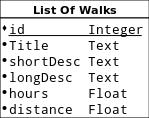
\includegraphics[scale=0.60]{Final_report/List_of_Walks.png}
\caption{List Of Walks Table}
\label{List Of Walks Table}
\end{figure}
In the list of Walks there is an if to identify the walk, this the primary key and all values are Unique. Next we have a title of the walk as a text field. Then we have a Short description of as a text field too, this has to be less than a 100 characters in length. Another field we have is the long description, which has to be to be less than 1000 characters. Finally, both hours and distance are of type Float. ~\\
~\\
	\indent\textbf{Location:}~\\\clearpage
	This table is where the user's co-ordinates, as either ``background'' co-ordinates are stored, or co-ordinates for the Point of interest during the walk. 
	\begin{figure}[htp]
\centering
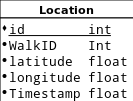
\includegraphics[scale=0.70]{Final_report/Location.png}
\caption{Location Table}
\label{Location Table}
\end{figure}
This table uses id as a unique primary key which is auto incremented and is of type integer. Another field in this table is the WalkId which is a foreign key references to Id in the list of walks - this is a foreign key as you will be able to keep track of which locations appear according to each walk. We then have latitude, longitude and a timestamp all as float representations. When the Android application records it will record background locations, so expect to have lots of co-ordinates in the table, that are not necessarily points of interest.

	~\\
	
	\indent\textbf{Place Description}~\\
	This table stores the description and name of any Location (Point of Interest) during the walk. Each Walk will be uniquely identified by the locationID
	\begin{figure}[htp]
\centering
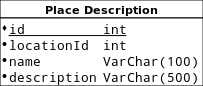
\includegraphics[scale=0.60]{Final_report/PlaceDescription.png}
\caption{Place Description Table}
\label{Place Description Table}
\end{figure}
This table refers to any point of interest during the walk. In this table you have a primary key called Id, which auto-increments every time a walk is added and is of type Integer.Then in the table there is the locationId, this is a foreign key reference to the key id, in the Location table - this again, is a way of keeping track of which point of interest is associated with a location and the co-ordinates for the point of interest. There is then a name and description which are both text fields in the database. These store the name of the point of interest and the description about the point of interest.
	~\\
	\indent\textbf{Photo Usage:}~\\
	This is the table which stores the photos for any given Point Of Interest. The table will allow multiple image for one location to be held as it stores the id for the point of interest
	\begin{figure}[htp]
\centering
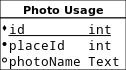
\includegraphics[scale=0.70]{Final_report/Photo_Usage.png}
\caption{Photo Usage Table}
\label{Photo Usage Table}
\end{figure}
In this table, we have a primary key Id for the photo which is auto incremented and uniquely identifies each photo in the table. PlaceID is a foreign key reference to the id in the place description table - again this is used to keep track of which photo is in which point of Interest. Finally, photoname stores the name of the photo minus the .jpg extension.
\paragraph{Algorithms}
All algorithms for inserting into the database is in file\_saver.php: This section is in the web maintenance section.
All algorithms for interacting with the database is in the list\_walks.php file, and walk\_details.php: These section is in the web maintenance section.
\paragraph{Main Data Areas}
There are no substantial data storage areas in the database as the database itself is the storage area. However when we get information from the database it returns it as an array. But this is covered in the Web Maintenance document.
\paragraph{Files}
There only needs to be one file in which the database is set up. This file is the C\_tables.php; as without this file the database will not be set up correctly. The user will then need to edit the Java source code to point the JSON Encoded values to the correct hosted area for the file\_saver.php which will then add the information to the database.
\paragraph{Interfaces}
The Database required MYSQL to be installed on the server. To view the tables then there are additional PHP files in the directory structure. 
\paragraph{Suggestions For Improvement}
An improvement which could be that the user would use software called PHPmyadmin. This would help greatly with having a visual representation of the database, as well as seeing the data in the database. This may help the user see it, rather than continuously using our PHP script.
\paragraph{Things To Watch Out For}
On our scripts we have added the Foreign Key References at the bottom of create table script, rather than under the actual value - so if the user is to edit this information and change any key dependencies then make sure that the last item is syntactically correct. Additionally, make sure that user chmod 700 the files - even though they're just SQL scripts inside, the file is .php - so you may not be able to run the script if the permissions are not set correctly.
\paragraph{Physical Limitation}
We think a physical limitation of our database is such: When the user uploads a walk, it retrieves the last ID key from the database and then increments it by one. Therefore, we feel that if a user tries to upload two walks simultaneously then we do not know what will happen. Thus, this leads to the potential issue of locking; where two users try to access the database at the same time.
\paragraph{Rebuilding And Testing}
To rebuild our database tables you simply have to firstly created a database to put the tables in to, from then you have to edit the mysqli\_connect parameters to your own host, your own username and password and your selected database. Then to create the tables you will simply have to run the c\_tables.php file; this will create the database for you and all the relations and dependencies.

To test the Database we have written a small PHP script/web page which allows you to view the tables and what information you have in them at any given time. There is also an additional file called d\_tables.php - this will allow you to drop all the data from the tables. \textbf{NOTE:} any tables which have been dropped will then be deleted, you will then need to call c\_tables.php again, to create the tables.

All tests to do with the database are in the Test Specification Document, under requirement: FR9 in the document. If the user wishes to edit this document then they will need to install a LaTeX editor,  and compile and build the document based on that software's documentation on how to do so. If the user wishes to add a new test, because of a fault then all they need to add the tests at the end of the test document by entering a test number, requirement, Test Content, Input, Output and a pass Criteria. They can do this in LaTeX by adding the \& symbol between each text data collumn - they can then finish it off by adding $\backslash \backslash$ to the end of the information - finally add a $\backslash$hline and this will complete the table. 
\newpage
\subsection{Personal Reflective Reports}
\subsubsection{Martin Vasilev Zokov}
The group project was an interesting experience from which I learned a lot. The task to make an Android application seemed a bit hard at first, but there are a lot of resources which help with understanding the problems we needed to deal with. I wanted to be one of the programmers on the projects so I was given tasks to implement some of the features in the Android application. During the process of developing the application, I learned a lot about the Android platform and how it works. Now I feel confident that I can use the knowledge gained to work on real projects for the Android platform.
~\\\\ 
Another great aspect of the group project is that I learned a lot about the way that commercial software is built. We were practically using the Waterfall model to implement our application and this gives insight into the way the industry works. I also improved my team working skills greatly, because the project concentrates heavily on collaboration between each member in the team. Not only about decisions that need to be made, but also when implementing certain aspects of the system, programmers should work with each other in order to create a working application.
~\\\\ 
The group leader (MDA) did a very good job with the task allocation and I feel that I was getting along with all of my team mates. We had no misunderstandings as a group and we worked pretty well in a team.
\subsubsection{Ryan Gouldsmith}
I feel that my contribution to this project has been extensive. First of deciding roles for the group was relatively straight forward, and although some people ended up being moved around to other tasks later on in the project to help with the lack of work being put forward, we all agreed that this was probably the best balance of skills in our group. I was delegated the role of Quality Assurance Manager, as well as helping with any issues to do with GitHub. Prior to the coding week, I was there to ensure that all the documents were adhered to by the standard specification that we received. As a group we all read the standard documents so we knew the outline for each of the documents that we were given. I thought we worked well as a team to help ensure that everything was to standard; overall, with the Quality Assurance I felt that we all worked together well and that standards were mostly adhered to.
~\\\\
However, around the Christmas period the Web Development team began to fall behind with the work. Therefore, Dave asked if I could assist in pushing forward with the Web site because it was falling behind - and as I had prior knowledge of HTML and PHP I was happy to do so. However, this continued into Integration and Testing week in which I had to code majority of the website - as the Web team may have been struggling to complete the work. I felt that the web programmers had done prior PHP courses at University, which wasn't too dissimilar from our group project, and I feel they could have done a little bit more towards the implementation.
~\\\\
I found my team very easy to get a long with, and we didn't have any overall major disagreements. I thought we all worked well as a unit, and we managed to discuss the different alternatives that we all decided. I think that we all made an effort to be there for our group meetings, showing we were all engaged in the project. I felt the most difficult aspect of the project was Integration and Testing week. I thought that this was a very long week, and trying to juggle 3 different aspects was very challenging; I had be QA to make sure if we edited docs they were still in standard, code the functionality of the website and help with the decoding of the JSON file from the Android. However, it was enjoyable being able to work as a team and when I didn't have not the correct solution someone could input: this was present with Dave's help with the multiple images on the website. 
~\\\\
From this project I feel that I have expanded additional web knowledge. Having only basic knowledge of PHP and JavaScript, it was good to be able to use this knowledge to produce an application which was flexible with the data that you gave it. I didn't however, have prior knowledge of how JSON worked, so having working decoding the JSON to put it into out Database was good and rewarding when we managed to be able to solve the issue, which stopped us for a couple of days. Additionally, the database design proved a bit of an issue as we were getting JOIN confused with foreign key, eventually we solved this and managed to sort out a database which is suitable to the design. However, I am happy I did manage to expand my knowledge on JavaScript and learning different programming techniques in the language: such as arrays and loops.
~\\\\
From the process I have learnt a great deal of useful information. I would happily work with my group again, but I feel that we could have potentially utilised the experience and confidence in programming a bit better. I would therefore have preferred to move to web development team from the start. However, I believe we have worked well as a team and I am happy with my contribution towards the final product.
\subsubsection{Zack Lott}
In CS22120 we was assigned a group project where we had to make a application and website.
We had weekly meetings with Neil about the progress of the application and website. This allows us to review the changes we did to the assignment. Our meetings were on a Friday at 10am but we occasionally had extra meetings with and without Neil to figure out what needed to be done to push the assignment forward. 
~\\\\
My role for this assignment was to be a tester, this meant I had to test the application and website, to check for bugs, errors and to make sure they met the requirements. I used the test specification that was created by the group with tests that were required, but with the web we used web validations and PHP unit testing.
~\\\\
From this assignment I have learnt new methods and ways of doing PHP from checking over the web code and creating PHP Unit testing, before this module I hadn't learn PHP unit testing so with the help of Dave(MDA), he helped me understand what it was doing and how to write/read it correctly. While doing the testing it made me understand the real purpose of testing, because checking the little things like checking for symbols in any text box can affect the whole application, this meant I spent a lot of my time while doing the works looking for ways that would break the application or make it crash, I managed to do this a few times but with that information our android workers put in a lot of effort and hard work to fix any problems I gave them.
~\\\\
The assignment did cause me a few problems but this was due to me not understanding many things due to me not studying 2nd part of Java in the first year, but Ryan(RYG1) and Dave(MDA) would quickly explain what it meant and how to solve the problem, this allows me to carry on with the work. If it was to hard then Dave would quickly reassign me something else so we could always keep the assignment going forward.  
~\\\\
I believe the group worked well, everyone got a lot with each other, we all had a laugh and they motivated me to work harder. Dave(MDA) was a great leader, you could go to him with any problem and he would drop everything to help try and fix it for you. Ryan(RYG1) was also a great vice-leader as he was always there if Dave was busy and was ready to step in if Dave was unable to attend the meeting. These both helped me with the assignment if I needed anything and they always made sure I was either testing or finding out information for them. 
\subsubsection{Jack Alexander Reeve}
My role in the team on this project was a web programmer / designer. This meant I was responsible for designing, building and populating the website. I mainly worked on this with Mark Pitman and Ryan.
~\\\\
Throughout this group project I feel as though I have made an acceptable contribution to the development of the system. In the design stages of the project I wrote up page descriptions for the website and made page designs in Adobe Photoshop. This work was used in the design specification document. I made a base template in HTML and CSS which was developed further into the finished design. In Integration and testing week I
spent a lot of time coding parts of the website. I feel that my knowledge of databases is a little limited so this made it difficult to work on pulling the walk details out of the database and listing it on the website. I worked with Ryan on this.
~\\\\
I was able to pull images from the database but I wasn't sure how to pull only the images corresponding to the correct walk. Towards the start of the week I worked on plotting points and drawing lines on the map using the Google Maps API. To start with, we just plotted points using dummy long and lat values. Then I worked on getting the JavaScript code to read these values from PHP variables so that the points plotted on the map were correct. I also worked on displaying POI descriptions and titles in the pop outs from the location pins.
~\\\\
Communication in the team was fairly good. We used emails to organise things such as group meetings. This was a method that was reliable as everyone in the team checks their university account on a regular basis. We had meeting at least once a week but often more, at locations and times suitable for all. Sometimes we worked on aspects of the project at these meetings but most of the time we worked on sections at home and
compiled them in the meetings.
~\\\\
Overall I feel we did well on the project as a group. We had a good spread of strengths which meant we were able to put in a good effort on all aspects of the project. We also had members with different skill levels which was good because it allowed other members of the team to learn.
~\\\\
I think if I was taking part in another project similar to this I would do more background research and learn more about the language I would be using. I had already worked with PHP, HTML5, JavaScript and CSS but not in as much detail as this project required. I should have researched specifically how to do what I needed to do well in advance of integration and testing week. Throughout integration and testing week I found myself having to research certain problems online. ~\\\\
I am fairly happy with the final system. We met the requirements and I feel that if we
had more time we would have been able to implement some extra features (such as
editing walk descriptions, deleting walks etc.) I also think we could have maybe
improved the look and design of the site, although it is functional and is all that is
needed for this purpose
\subsubsection{Mosopefoluwa David Adejumo}
For the CS22120 Group Project, I had the role of group leader. I chose this because I had experience leading teams and had knowledge of both web and android development.~\\\\
Initially, I found the role somewhat difficult, particularly in keeping all group members engaged and keeping the project on schedule. To assist me in monitoring the progress of all members, and ensure all members were contributing, I requested all members produce weekly reports which would be a summary of the work done in the last week and later on the reports would be a summary of the blog. This was useful in monitoring the amount of time each member spent on the project. ~\\\\ 
The reports were also useful for monitoring areas where members had problems. Weekly group meetings were arranged early and I made sure all members were kept up to date with proceedings of each meeting. Many issues were brought up during meetings by or with our project supervisor some of which would be solved during the Friday meeting. ~\\\\
I found the prototyping slow on the website end and decided to break work down into individual pages for the web prototyping. Despite initial setbacks, the members were generally responsive with instructions and I found, the carried out the tasks relatively quickly. The only issues I found serious was the lack of web development over the Christmas holiday and I lost contact with the web programmers and thus asked the quality assurance manager to begin development on the website. I ensured all members were able to contact me with ease particularly with issues. ~\\\\ 
I found pre-assigning tasks for coding week somewhat difficult due to my inability to determine how easily a task would be accomplished, however I did find it fairly simple to do overall planning and set milestones. The project supervisor suggested I use hour based deadlines/timeframes for project tasks. I found this difficult and the group members preferred our existing system whereby deadlines were set on specific days. I.e. instead of spending a limited number of hours on a task, the task would have to be completed by a particular day. This system worked for the members. The project supervisor also suggested involving more group members, but the group members and I wanted to avoid this as it could compromise the system which we had and was working as required. ~\\\\
Overall I think the group performed well and constantly kept me up to date with all progress made. They would quickly work on a task that I instructed and lack of technical knowledge was the main barrier to accomplishing tasks. If they had issues they would keep me informed and also notify me about problems. I found it easy to explain certain areas to them, though there were issues of misinterpretation of instructions or statements. If they had issues it was easy to solve and while there were situations where several members would have problems, the members were very intuitive at solving them. This allowed me to assist multiple members in a short space of time and thus keep development on schedule.~\\\\
I did find several members putting in more effort than others, though this was possibly due to the different areas they worked on and the fact that some members did not understand certain concepts which was brought to my attention and thus, I believe the members cannot be faulted as they would quickly pick up work were problems were encountered. I made several jokes to keep the mood light hearted and keep morale high, which had effects as there were times particularly during integration and testing week when members became overly burdened with work and thus I would instruct them to rest as required while I took up the task they had issues with in an attempt to solve them.~\\\\
I learned a lot about the importance of feature creep identification during the project and the importance of communication between all the members and feel my team performed extraordinarily well.
\subsubsection{Mark Radcliffe Pitman}
The group worked well together and there were little arguments, which was good. Everyone had there role and stuck too it. ~\\\\
My role was the web part. Mostly CSS but helped with the HTML and PHP too. I attended most meeting with the tutor and our general meetings. I missed 2 or 3 meetings for good reasons.  We had meeting every Friday at 10am. Occasionally we had extra meeting if something needed to be sorted. ~\\\\
I learnt a lot for this project from working with a group and more knowledge on HTML, PHP and CSS. I researched a lot on PHP and the assignment I did for web helped a lot. Also learnt a bit from the android side. It felt good once everything was done and everyone's work came together. When seeing the app uploading to the database and it shows on the website felt fulfilling.  ~\\\\
The leader did a very good job keeping everyone busy and telling everyone what needs to be done and by when. Was very supportive and tried to help everyone with their jobs if they needed help.~\\\\
We did have problems like the website wasn't receiving from the database and show on the map. Problems with the images to show up. The info box sometime didn't show what we wanted. The CSS could mess things up with the texts, for example, making the page smaller, the words would move around where they shouldn't be. This was all fixed after other people started helping each other cause they finished their part of the job. This showed good teamwork. ~\\\\
Personally I enjoyed working as a group. I felt more motivated cause I didn't want to disappoint the group. If something wasn't done then it just doesn't affect you but the whole group.~\\\\
 There were some stressful moments when things weren't working but that was expected. Nothing was really left to the last minute because the leader wanted things to be done some time before the deadline so it can be checked and changed. Glad everything went mostly well and it
is finally done.
\subsubsection{Mark Alexander Smith}
Our CS22110 module involved us being part of a nine-person team and creating an android application about walk tours. It would involve the application using GPS on a users phone, saving the details (co-ordinates, description and images) of that users walk; this would link to a database. This information could then be sent to a website which would display all of the users walks.~\\\\ 
Our first meeting involved us deciding roles for our team. We decided that David should be our project leader; he was enthusiastic about taking up this role. Ryan took up the role as being QA manager. Martin and Harry both took the roles of being android developers. Myself, Jack and Mark P took the roles of website developers, myself creating the database. Zack and Maciej accepting the roles of being android and PHP testers.~\\\\
Our group would meet on a regular basis, every Tuesday with our Tutorial Tutor, Neil Taylor.  We would then also meet together as a group once or twice a week in our own time, usually in the orchard or the old college in town. I think this gave us an edge over other groups as each week we would all attend and discuss any problems we had, and create new jobs before we visit Neil later in the week. Obviously not everyone could make every session due to other commitments, but communication between the group was good enough so that this happened as little as possible.~\\\\
We were in a good position leading up to Integration and Testing week (ITW), however this week is where most of the work would get done. I started on working with Ryan on the filesaver.php file. This became an issue with the group and became a harder task to do than first project and therefore took a lot longer than first suggested. Later in the week I continued with the website by creating the base of the CSS and also helping out with some problems, and also taking out some testing of the android application.~\\\\ 
Overall I believe that our group took the correct attitude towards such a big project and getting as much done as possible before ITW. Meeting in our own time took a big weight off our shoulders and lead us to getting a working application that would send information to the database and website. David lead us well in making sure deadlines were met and that we were up-to-date on the Gantt chart.
\subsubsection{Harry Flynn Buckley}
During this task I occupied myself with the Android-server communication and general handling of the walk data on the device. I feel that I am largely responsible for the class design of the Android application, and although towards the end the project it had to stray a little from the initial design, due to unforeseen complications with the Android camera and gallery apps, I am still happy with majority of the design choices. As there were only two people programming on the android, I had quite a lot of input to all the aspects of the android, the pop up dialogs where the only area which I feel I only had little contribution. 
~\\\\
The group worked quite effectively, discussing much of the design before making a decision, I do however think that class diagram was not looked at very thoroughly as I received little feedback on my designs. I think the UI design perhaps had too much focus in the early meetings because UI is something that is very accessible and everyone has an opinion on. When the implementation part of the project started I wrote the initial GUI based on what was decided by the group, this went on to become the GUI of the final submission. I then worked on writing the all the model classes (WalkModel,LocationPoint,PointOfInterest, ImageInformation). A feature that was eventually cut was a local sqlite database that stored walks before they where uploaded, I managed to get the database working with much of the walk data but it was not complete.The next task that I was set on was the uploading of walk data to the server, this was initially done in name value pairs, before we decided on using JSON. To test the upload I had written a php file that receives and saves the send data and I think this file contributed to the final file\_saver.php. During ITW I finished off the JSON packaging, and did  all the camera and gallery interaction. I had some trouble writing the camera and gallery, as it involved slightly redesigning the way images are stored and how places of interest are added to the walk model. The packaging of the walk data into a JSON format was also quite difficult.
~\\\\
Overall I have found the process quite fun and exciting, more so the closer we got to the code hand in date.
\subsubsection{Maciej Wojciech Dobrzanski}
At the beginning of the project, we were assigned to certain roles. I was supposed to be a designer, tester and a person responsible for the documents. We also decided that we can all help each other with our tasks to make everything easier and more convenient. At the beginning I had quite a lot of work, which I feel I've done pretty well. I was delivering everything on time, was also trying to help others with their parts of the design, because a team of designers was supposed to work together to create a really specific design. To sum up, the first part of my work was done just as planned and I feel like I couldn't really do anything more than that. I certainly could work on a couple of things faster, to allow others to use my work, but no one really needed that. 
~\\\\
 I was also supposed to work on the Use Case and UML Diagrams. We had quite a few ideas of how they should look like, I was trying to gather and improve them. I've learned quite a lot about the UML Diagrams, which were not really my strong side. The use cases were designed quite well, we thought it might be a good idea to add a few features to the project to make it more appealing, so the changes were clearly visible on the diagrams. The coders helped me develop a good diagram. Although the use cases were not a big issue and they were ready really quickly, I was really worried about the UML diagram as it took me a really long time to come up with the idea of how it should look like. I knew that the coders were not able to start working because of me, and I was trying to figure it out as soon as possible, to give them more time on the project itself. 
~\\\\
After the design specification was ready, I did not really have a lot of work to do. I was trying to help the coders with the Android application, but the Android Java code was a little bit different than a normal Java code, so it was quite difficult for me. The group asked me to work on a Git Wiki. I managed to catch a few things of how to write it pretty quickly and spend about a week developing it. I think it wasn't really good as my overall knowledge of the project details was quite shallow, everyone had to add a few things from their own experience during development of the project. I was really struggling with it because I didn't really see a point in doing it – I didn't see how it could be useful.
~\\\\
When I came back from the Christmas break, I reviewed all of the documents we've prepared and I tried to catch up with the current state of the project to be able to spend my time well during the coding week. When I was really able to do my part(which was testing) I tried to help everyone else created JUnit tests, was helping the coders and doing a little bit of all-around help, asking other group members if they needed any help. I did all I could with the documentation when there was nothing else to do. The first plan was that I am supposed to write the final documentation, but when the coding week was coming to an end, we all knew that one person just cannot do that, it will have to be a group effort, as everyone did something else and no one really had a deep knowledge of every single part of the project.
~\\\\
To conclude, I've learned a lot during the group project. I was trying to do as much as possible to be an important group member, but sometimes I had an impression that everything is taking too much time and the group won't be happy with my work. I would like to think of myself as a valuable member of the group who was always able to have something to add and was always able to help others, but the truth is that sometimes my knowledge was just not enough and I was not satisfied with myself. On the other hand, I always managed to do anything that I was asked to do, even if that required more work and researching things that I've never seen before. I had a lot of fun and the whole project helped me develop not only as a person, but also a good future employee.
\newpage

\subsection{Revised Project Plan}
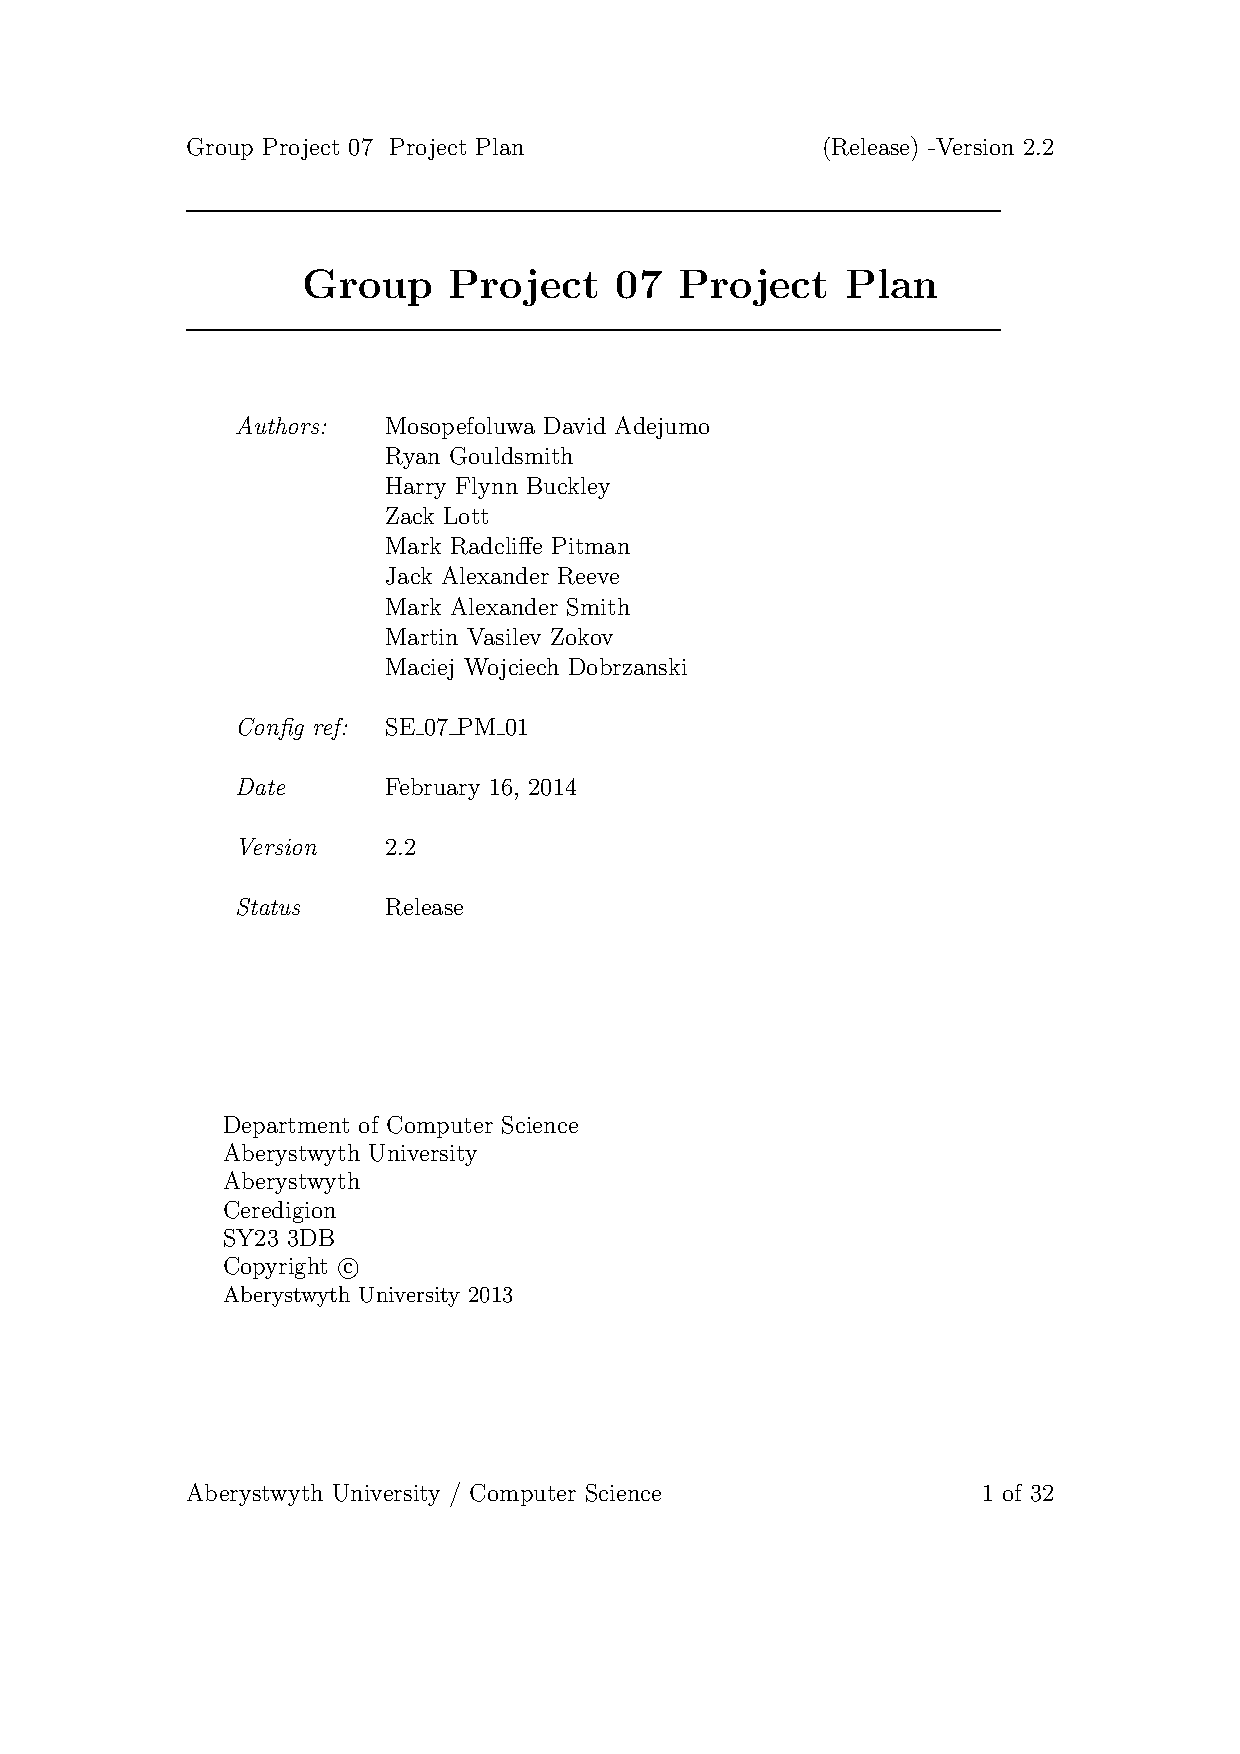
\includepdf[scale=	0.95, pages={1-27}, pagecommand={}]{ProjectPlan.pdf}
\newgeometry{top=1.5cm, bottom =1.2cm}
\includepdf[scale=	0.95, pages={28}, pagecommand={}, landscape=true]{ProjectPlan.pdf}
\restoregeometry
\includepdf[scale=0.95, pages={29-33}, pagecommand={}]{ProjectPlan.pdf}



\subsection{Revised Design Document}
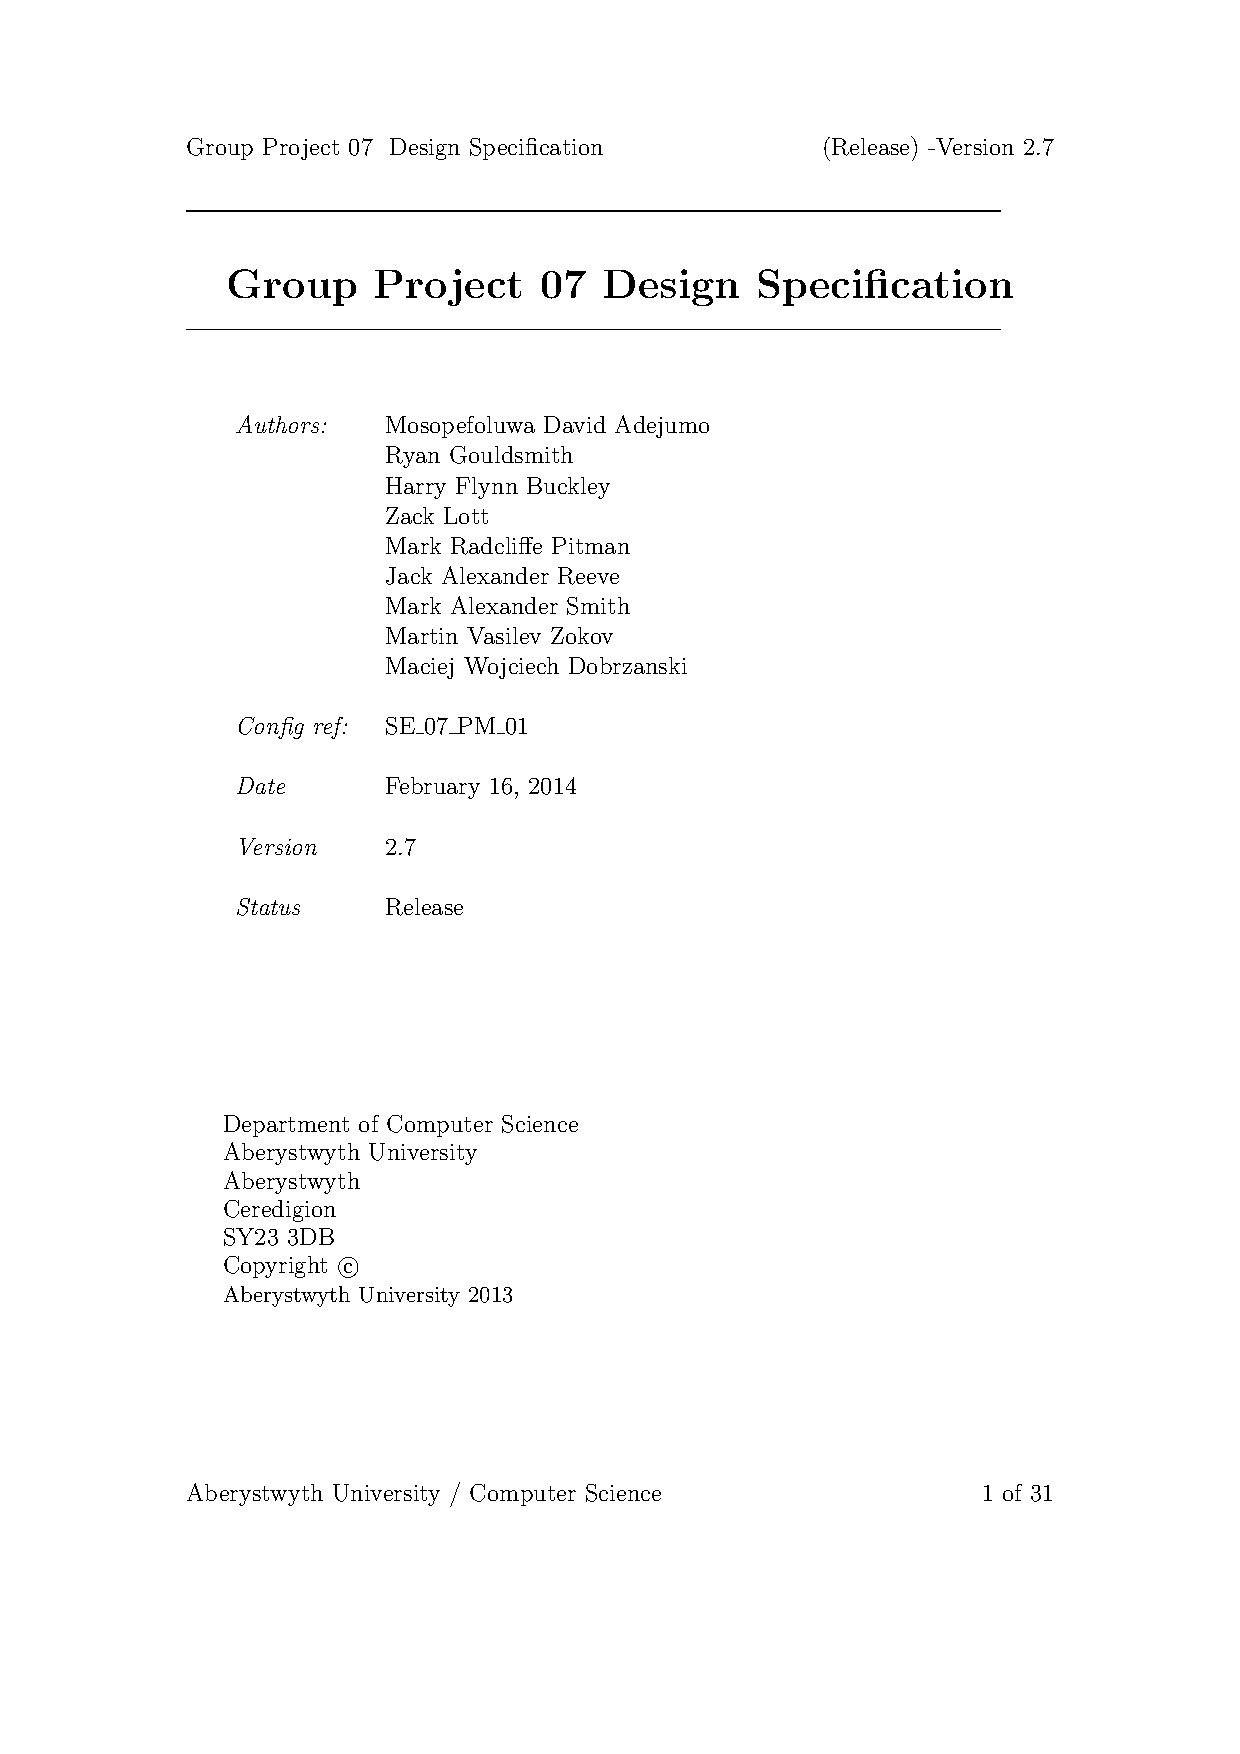
\includepdf[scale=0.95, pages={1-24}, pagecommand={}]{DesignSpec.pdf}
\newgeometry{top=1.5cm, bottom =1.2cm}
\includepdf[scale=	0.95, pages={25}, pagecommand={}, landscape=true]{DesignSpec.pdf}
\restoregeometry
\includepdf[scale=	0.95, pages={26-}, pagecommand={}]{DesignSpec.pdf}


\section{REFERENCES}
\begin{thebibliography}{0}
\bibitem{Design Specification 2.9}
Software Engineering Group Projects
\emph{ Design Specification}.
M.D. Adejumo, CSGroup - 7 Members 2.9
(Release). 17th February 2014
\bibitem{Project Plan 2.5}
Software Engineering Group Projects
\emph{Project Plan}.
M.D. Adejumo, R. Gouldsmith and others 2.5
(Release). 17th February 2014
\bibitem{Test Specification 2.8}
Software Engineering Group Projects
\emph{ Test Specification}.
M.D. Adejumo, R. Gouldsmith and others 2.8
(Release). 16th February 2014
\bibitem{Requirements Specification 1.6)}
Software Engineering Group Projects
\emph{Walking Tour Creator Requirements Specification}
C. J. Price and B.P.Tiddeman 1.6 (Release). 29th January 2014
\bibitem{Earth Image}
Abcteach Earth-image Internet:http://www.abcteach.com/free/e/earth\_3d\_rgb.jpg [28 Jan 2014]
\bibitem{Pencil Project}
Pencil Pencil Application Internet: http://pencil.evolus.vn/[17 Feb 2014]
\bibitem{Paragraph}
lockstep Paragraph LaTeX formatting~\\Internet: http://tex.stackexchange.com/questions/4891/how-do-i-control-the-spacing-above-a-new-paragraph[14 Feb 2014]
\bibitem{Real Path}
m3n0R File paths of images \\ Internet: http://stackoverflow.com/questions/2789276/android-get-real-path-by-uri-getpath [25 Jan 2014]
\bibitem{Distance Calculator}
Distance calculator ~\\ Internet:http://stackoverflow.com/questions/837872/calculate-distance-in-meters-when-you-know-longitude-and-latitude-in-java [26 Jan 2014]
\bibitem{Lightbox}
Lightbox Lightbox application~\\ Internet:http://lokeshdhakar.com/projects/lightbox/ [24th Jan 2014]
\end{thebibliography}
\newpage
\section{DOCUMENT HISTORY}
\setlength\LTleft{-0.5cm}
\begin{longtable}{|p{1.3cm}|p{1.5cm}|p{2cm}|p{7cm}| p{2cm}|}
\hline
	Version & CFF No. & Date & Section Changed From Previous Version & Changed by \\
\hline
	1.0&N/A&13/02/2014&Set the Original Document Layout&RYG1
 \\ 
\hline
	1.1&N/A&13/02/2014&Added other team members reports.&RYG1 \\
\hline
	1.2&N/A&13/02/2014&Added new reports and made small edits.&MDA \\
	\hline
	1.3&N/A&13/02/2014&Added new reports and Android maintenance details.&MDA \\
\hline
	1.4&N/A&13/02/2014&Moved the Maintenance to the correct section of the document. Added the Web Application maintenance report.&RYG1 \\
\hline
	1.5&N/A&13/02/2014&Text correction. Added new paragraphs.&MDA \\
\hline	
	1.6&N/A&13/02/2014&Added the Database Manual Section&RYG1 \\
\hline
	1.7&N/A&13/02/2014&Added more information to the Database manual&RYG1 \\
\hline		
	1.8&N/A&13/02/2014&Added more information to the Android manual&RYG1 \\
	\hline
	1.9&N/A&13/02/2014&Grammar, syntax and spelling corrections. Capitalized user names. Updated system interaction and added use case descriptions. Added maintenance docs for field form and add fields PHP files.&MDA \\
	\hline
	2.0&N/A&13/02/2014&Updated Version numbering.&RYG1 \\
	\hline
	2.1&N/A&13/02/2014&Formatting issues fixed. Updated evaluation &MDA \\
	\hline
	2.2&N/A&17/02/2014&Added Test Log &RYG1 \\
	\hline
	2.2&N/A&17/02/2014&Edited some typos&RYG1 \\
	\hline
\end{longtable}

\end{document}